\section{Class Diagrams}
A class diagram describes the structure of a system by highlighting the 
system's classes, attributes, methods, and relationships among other classes 
\citep{lunn03}.

Within this section a number of class diagrams will be presented. Each class 
diagram will represent a namespace (used to declare a scope, similar to a Java
package) in order to simplify the representation of classes. 


\subsection{Namespace Overview}
Figure \ref{fig:NSOverview} is a general overview for all the namespaces within
the system. 

Each namespace will contain specific code that is related to a certain part of 
the system's functionality. Each namespace will be compiled into a Windows 
Dynamic Link Library file (.dll). 

This will ultimately allow for re-usability for other future projects or 
extensions.

\begin{figure}[H]
  \centering
    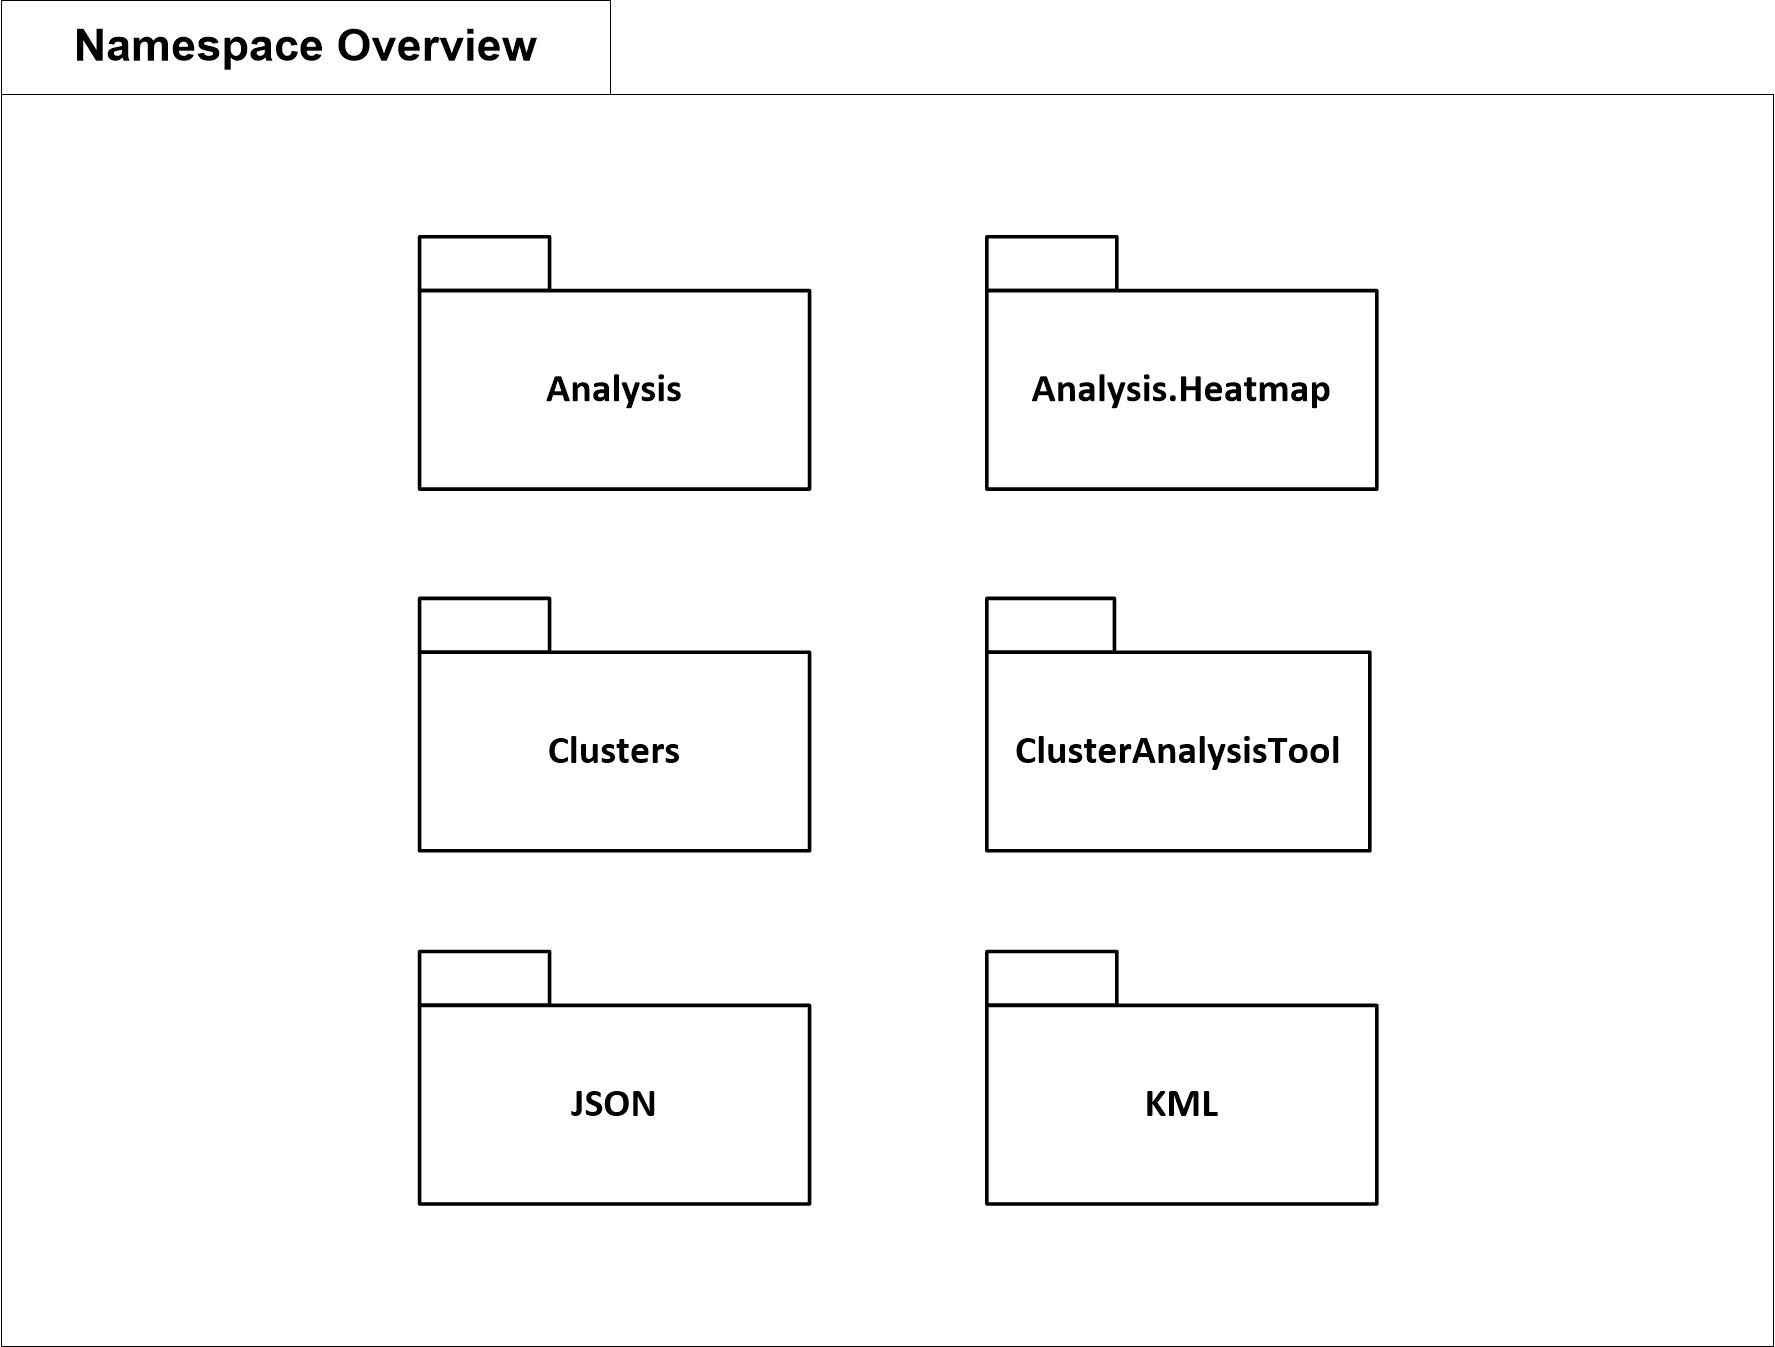
\includegraphics[scale=1.0]{chapter7/class_diagrams/namespace_overview.png}
    \caption[Overview of the entire Cluster Analysis Solution]
            {Overview of the entire Cluster Analysis Solution.}
    \label{fig:NSOverview}
\end{figure}



\subsection{Analysis}
Figure \ref{fig:NSAnalysis} shows the Analysis namespace, which provides the 
system with all the analysis classes, business logic and template output files. 

The Event Analysis class is an abstract class (indicated by the italic name), 
which is able to to provide generic functionality to analyse Drop and Fail 
events. Any additional Drop and Fail analysis will placed into these classes.
It is these classes that provide analysis upon one type of event within one
cluster.

The Cluster Analysis object is the main entry point for analysing a given 
cluster with a set of clusters. This class provides functionality to directly 
make use of the methods found within the DropAnalysis and FailAnalysis classes.

The Analysis class is another abstract class than provides analysis for a group 
of clusters. The Product Analysis and Week Analysis classes extend the Analysis
class to provide four specific forms of analysis. 

By utilising both the DropAnalysis and FailAnalysis classes, the Product 
Analysis and Week Analysis classes are able to analyse an entire product or 
week respectfully.

The AnalysisResults and AnalysisResultsCollection classes are alias classes for
complex dictionary objects. Both of these classes will store the results 
generated by the analysis classes as key/value pair lists. 

The JSON results class stores a number of AnalysisResultsCollection objects for
easy converting to a JSON format.

The MultiAnalysis class provides a base class for different forms of analysis 
to easily happen. The MutliWeekAnalysis class extends the MultiAnalysis class, 
which allows for easy access to analyse all the given weeks (or an individual 
week). 

This class possess functionality to output all analysis as a JSON string or as 
a JSON file.

\begin{figure}[H]
  \centering
    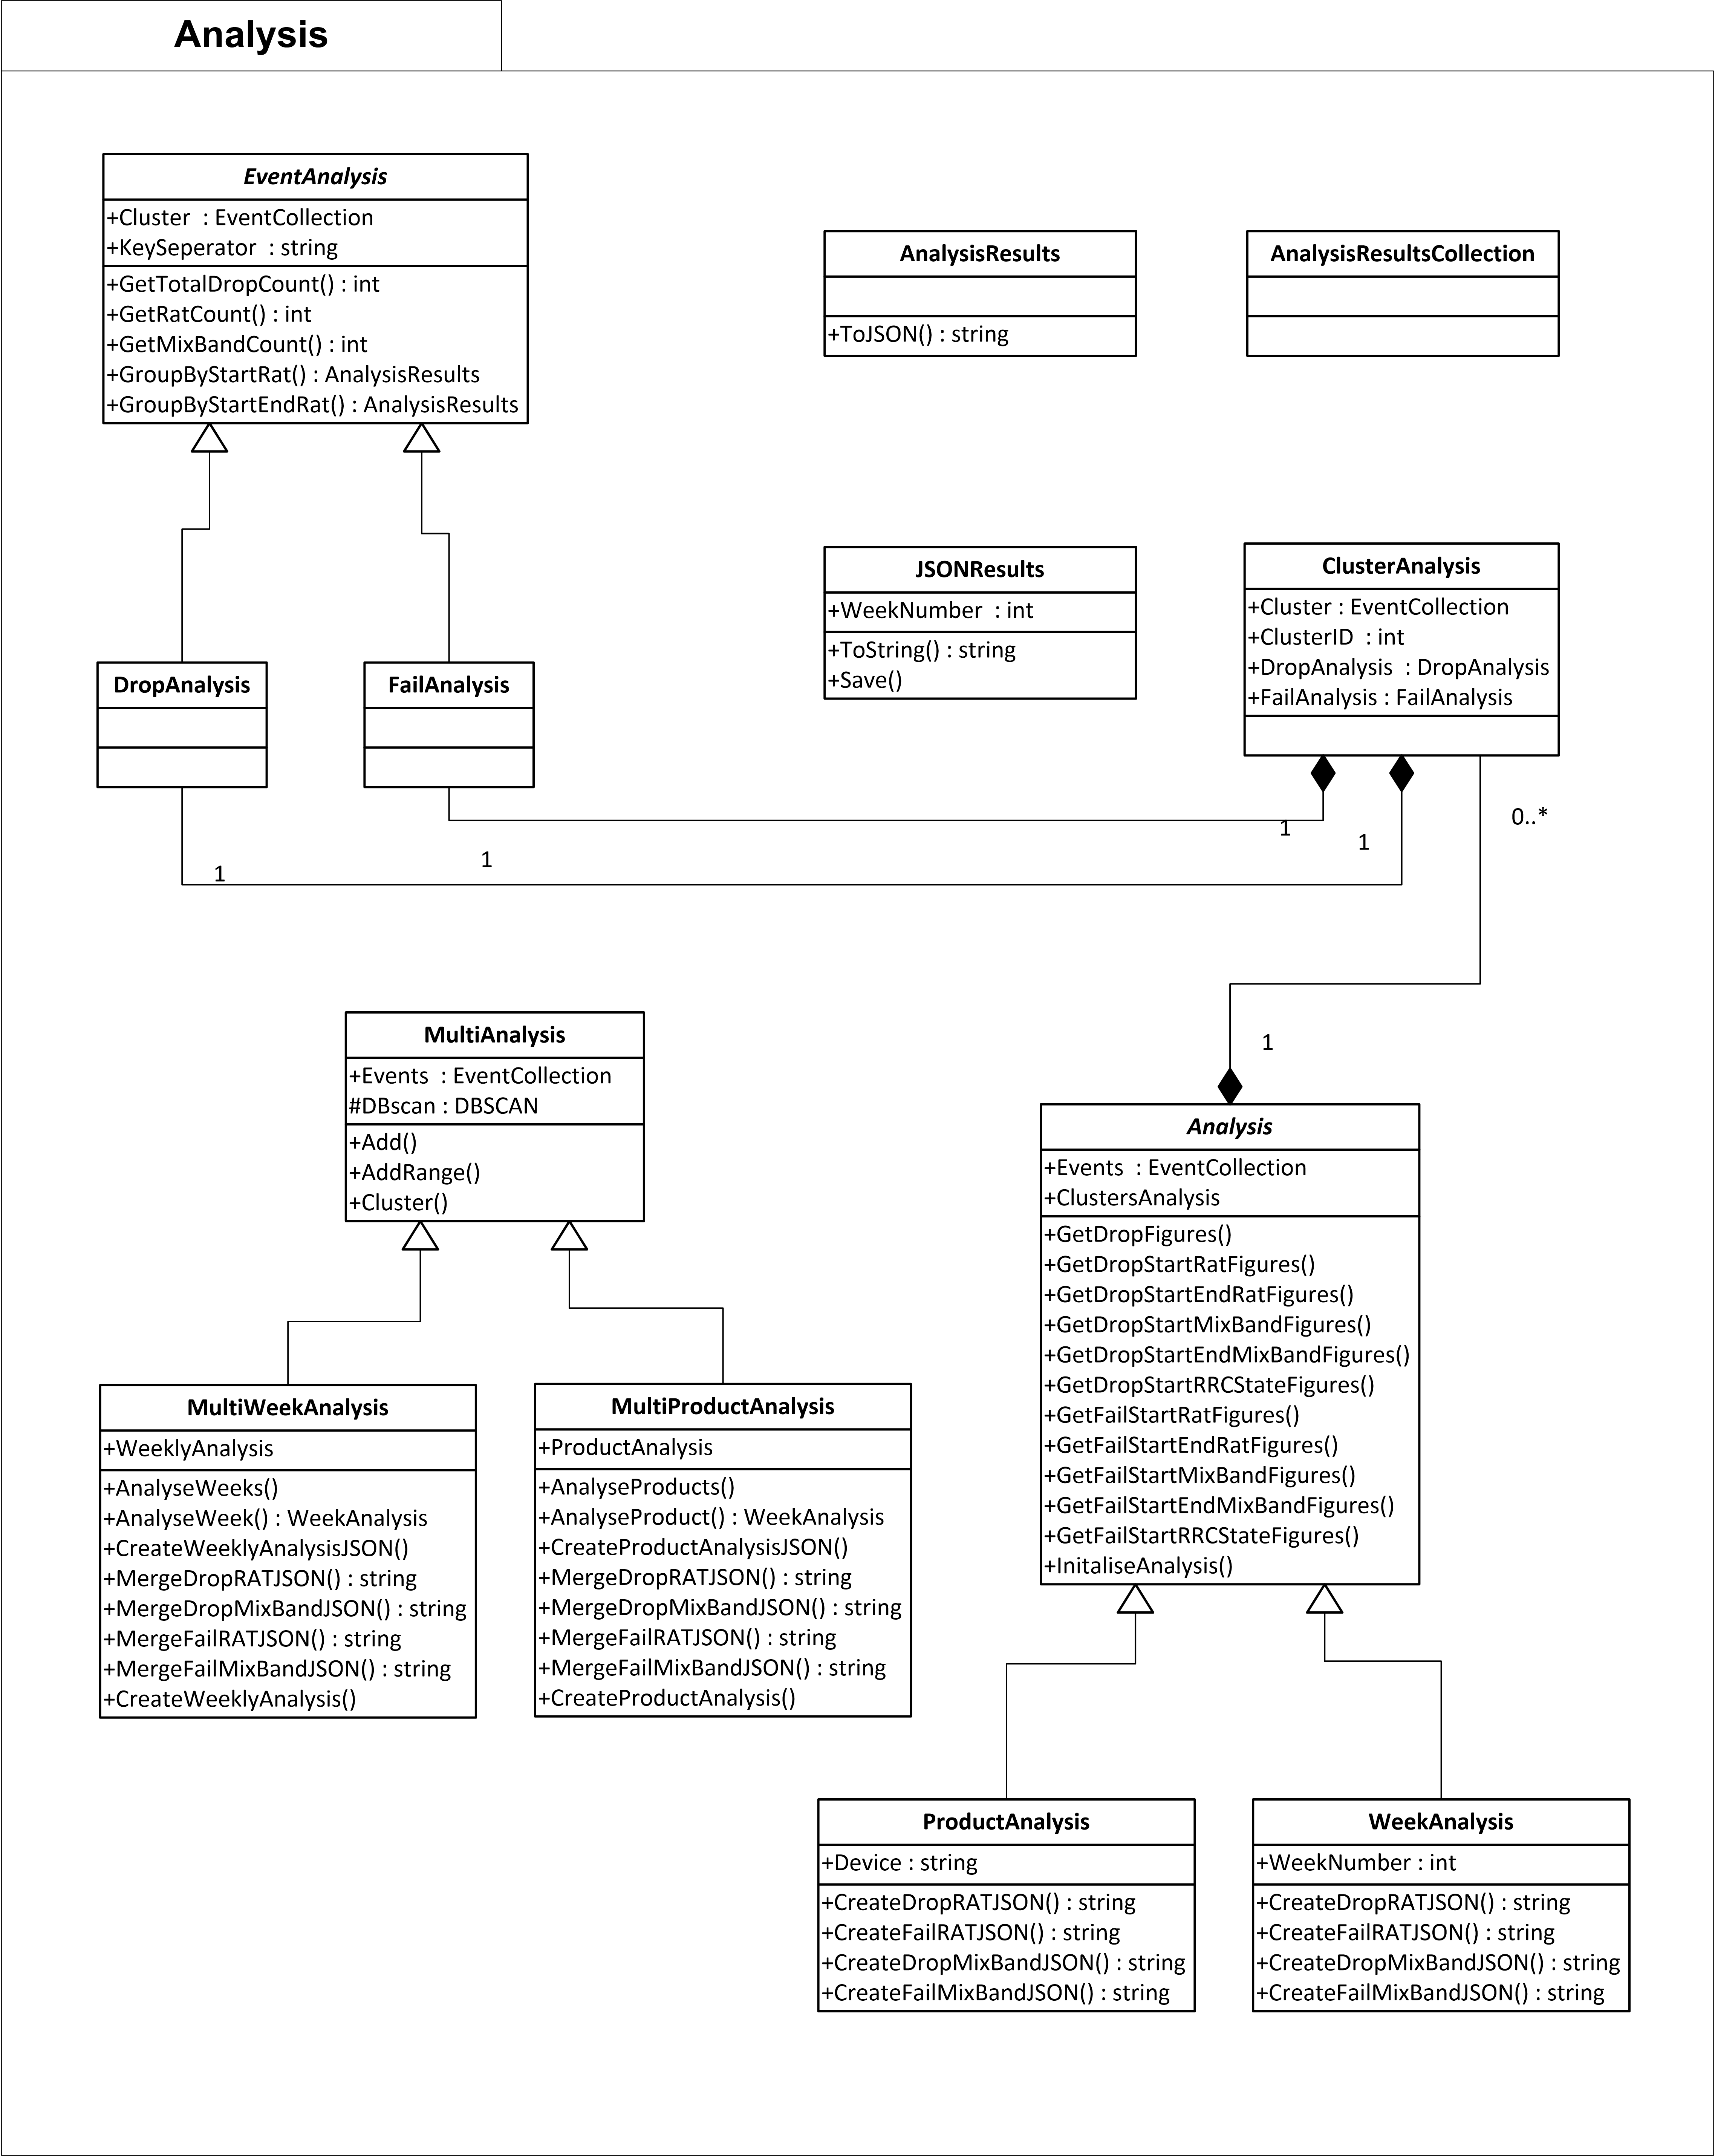
\includegraphics[scale=0.8]{chapter7/class_diagrams/analysis_namespace.png}
    \caption[Analysis namespace class diagram]
            {Analysis namespace class diagram.}
    \label{fig:NSAnalysis}
\end{figure}



\subsection{Analysis.Heatmap}
Figure \ref{fig:NSHeatmap} shows the Analysis.Heatmap namespace, which is a 
sub namespace of the main analysis class. This namespace provides functionality 
to allow for heatmaps to be created. to highlight high object intensity upon a 
map.

The Heatmap class is the main entry point to create a heatmap. The class will 
convert an EventCollection a collection of HeatPoints. The conversion involves 
mapping a GPS coordinate to a screen coordinate, and assigning it an intensity 
weighting. 

The ColorScheme class will provide a set number of colour schemes, to allow for 
the user to change the colour scheme of the heatmap.

\begin{figure}[H]
  \centering
    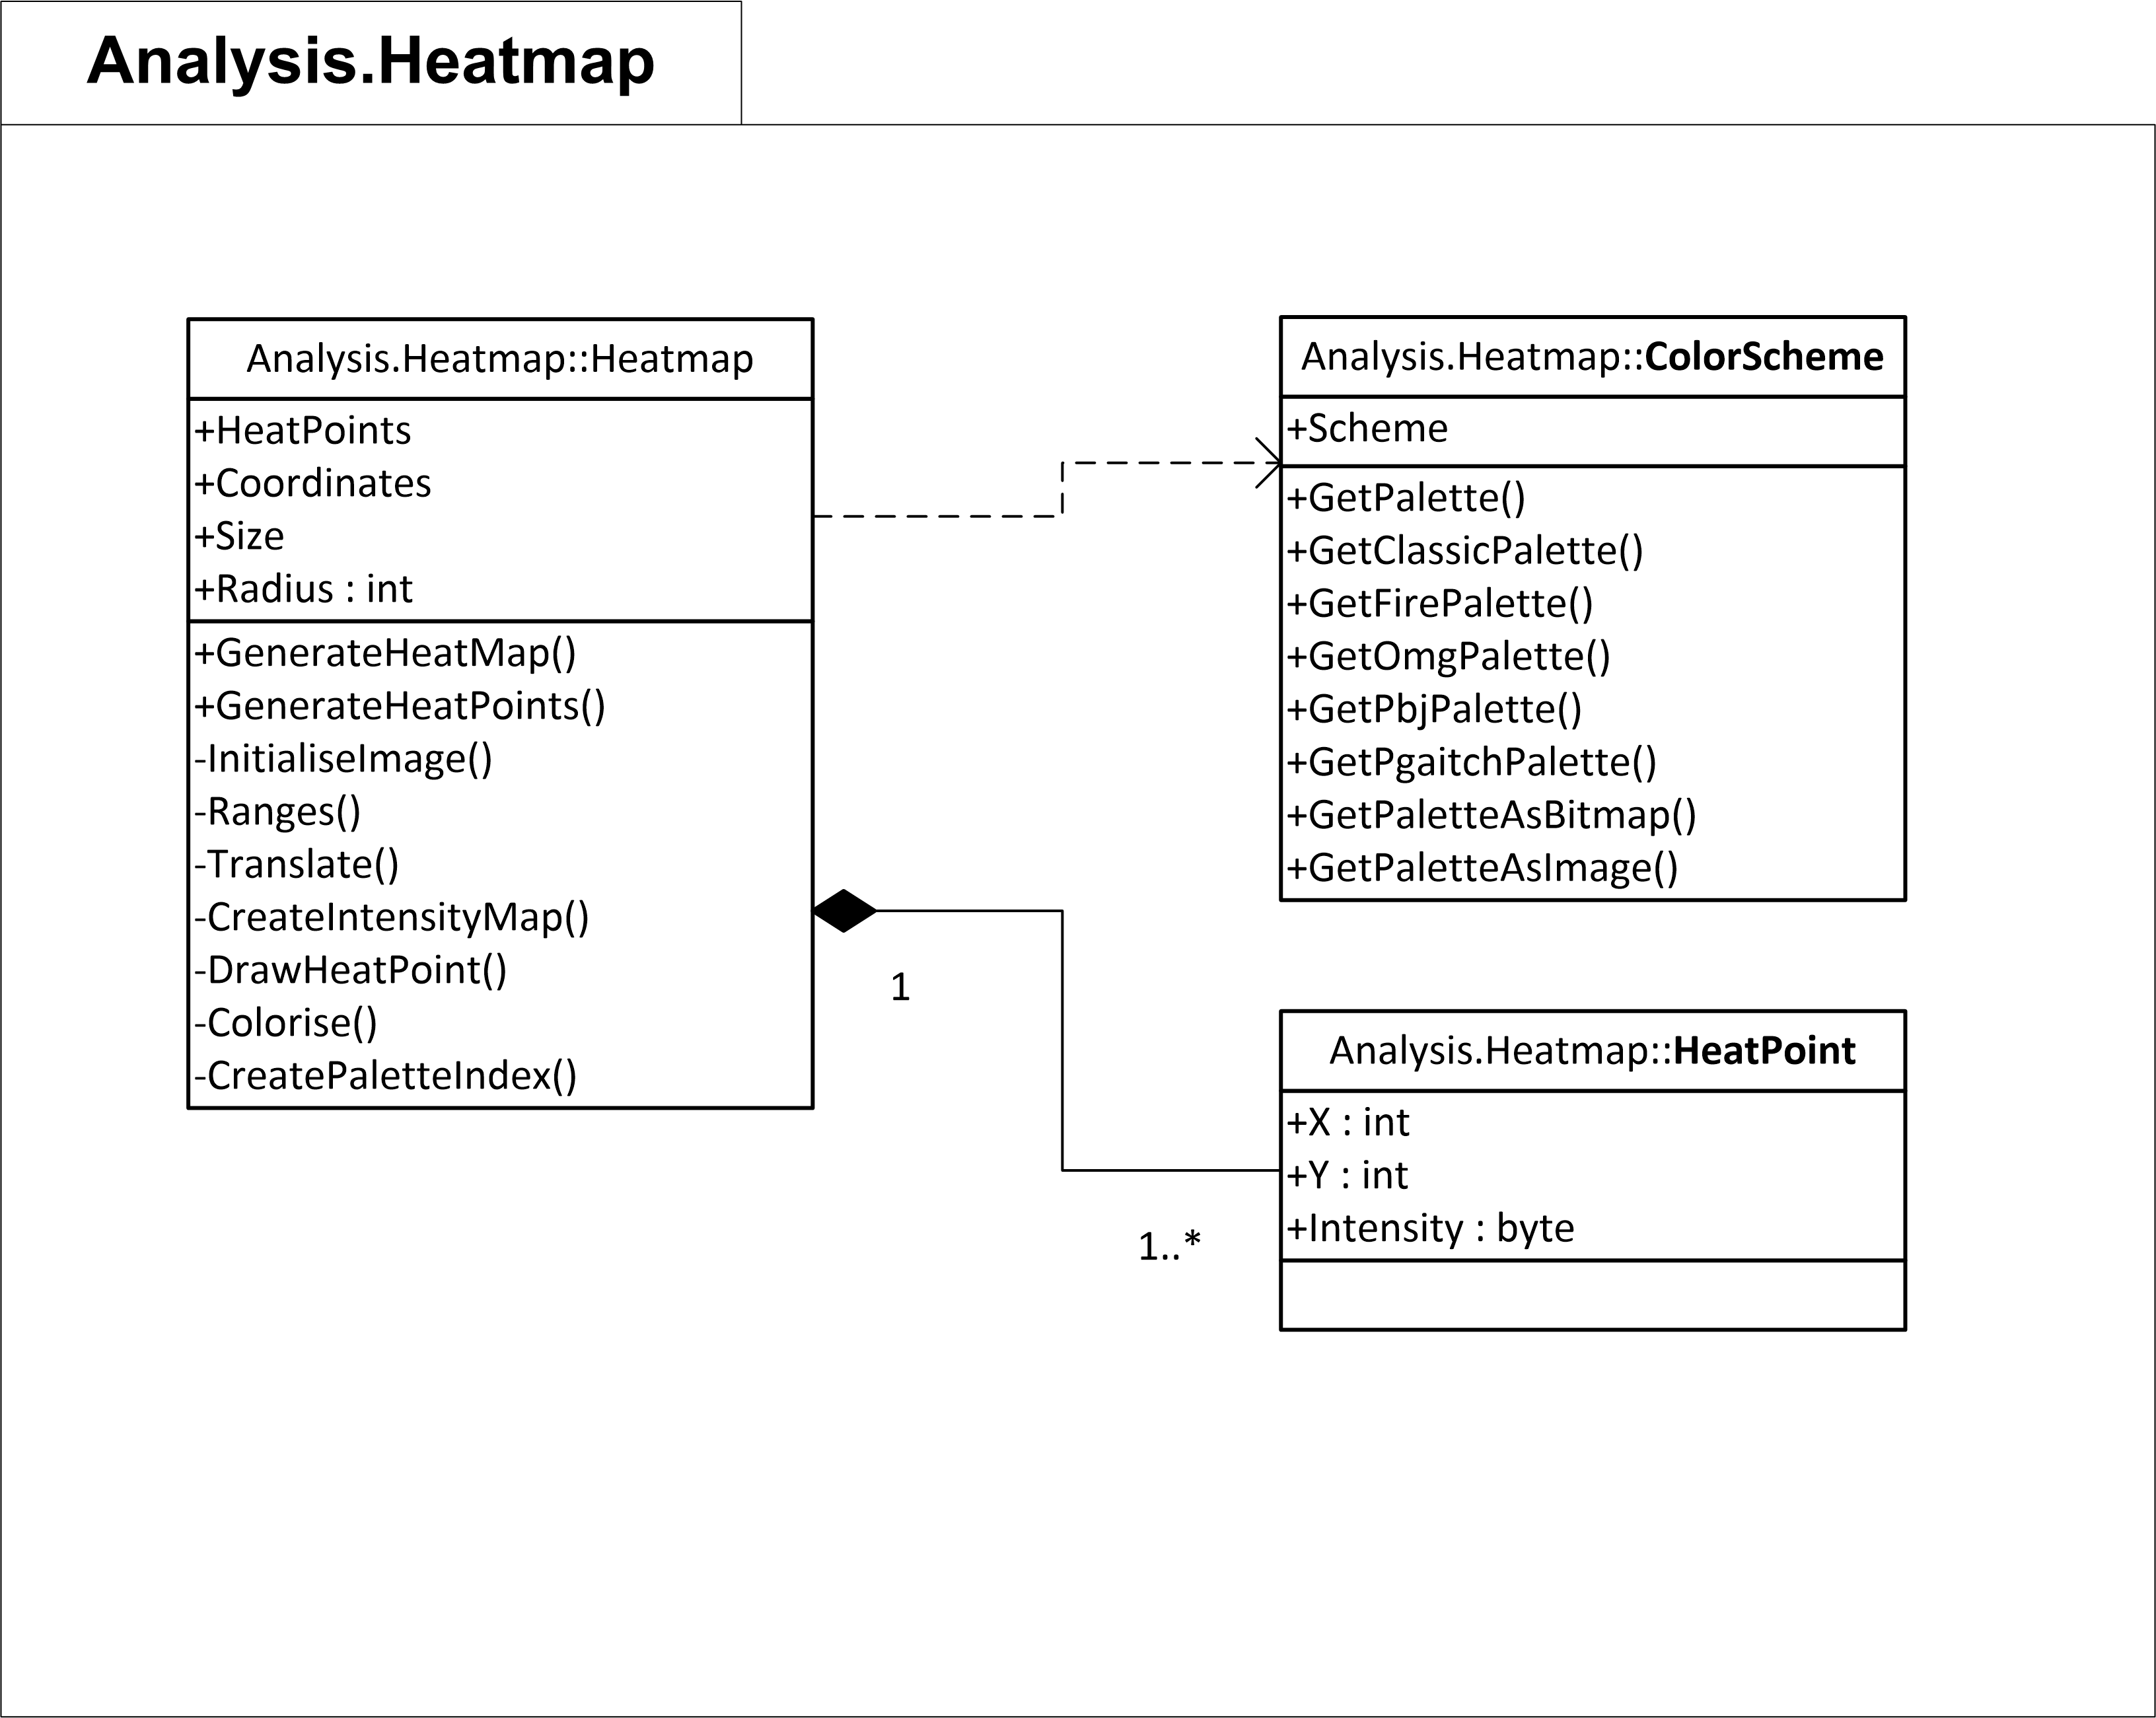
\includegraphics[scale=0.9]{chapter7/class_diagrams/analysis_heatmap_namespace.png}
    \caption[Analysis.Heapmap namespace class diagram]
            {Analysis.Heatmap namespace class diagram.}
    \label{fig:NSHeatmap}
\end{figure}



\subsection{Clusters}
Figure \ref{fig:NSClusters} shows the Clusters namespace, which provides the 
system with the ability to cluster events. Additional fundamental classes such 
as Events, Coordinates and their respected collections can also be found within
this namespace.

At the simplest level, the Coordinate class represents a GPS Coordinate, along 
with some additional values that are used by the clustering algorithms. The 
Centroid class extends the coordinate class to add the radius field, which holds
the size of the radius. 

The Event class is an abstract class that models a given event. Additional 
details such as device, pin, timestamp etc are stored along with the Coordinate 
of the event. The event class can not be directly instantiated, and thus there 
are a number of classes for each type of event, Fail, Success and Drop.

The EventCollection and CoordinateCollection both extend the List, to allow for 
any number of events and coordinates to be stored in a collection. Events and 
coordinates can not be mixed up in the same collections. Each collection 
provides the same methods, that allow the elements to be manipulated easily.

The RadialCircle class allows a radius to be draw around a given point, with a 
given radius. The SphericalCoordinate provides additional support for this 
feature. The Distance class is a static class that calculates the distance 
between two given coordinates based upon a number of formulas. Each formula has 
a different accuracy level.

The DBSCAN and K-Means classes both provide an implementation to the DBSCAN and
K-Means algorithms respectfully. Each take either an EventCollection and return 
a List of EventCollections. Each element within the list represents a cluster. 
The DBSCAN class has an additional field which stores events and coordinates 
that are deemed to be ``noisy''.

\begin{figure}[H]
  \centering
    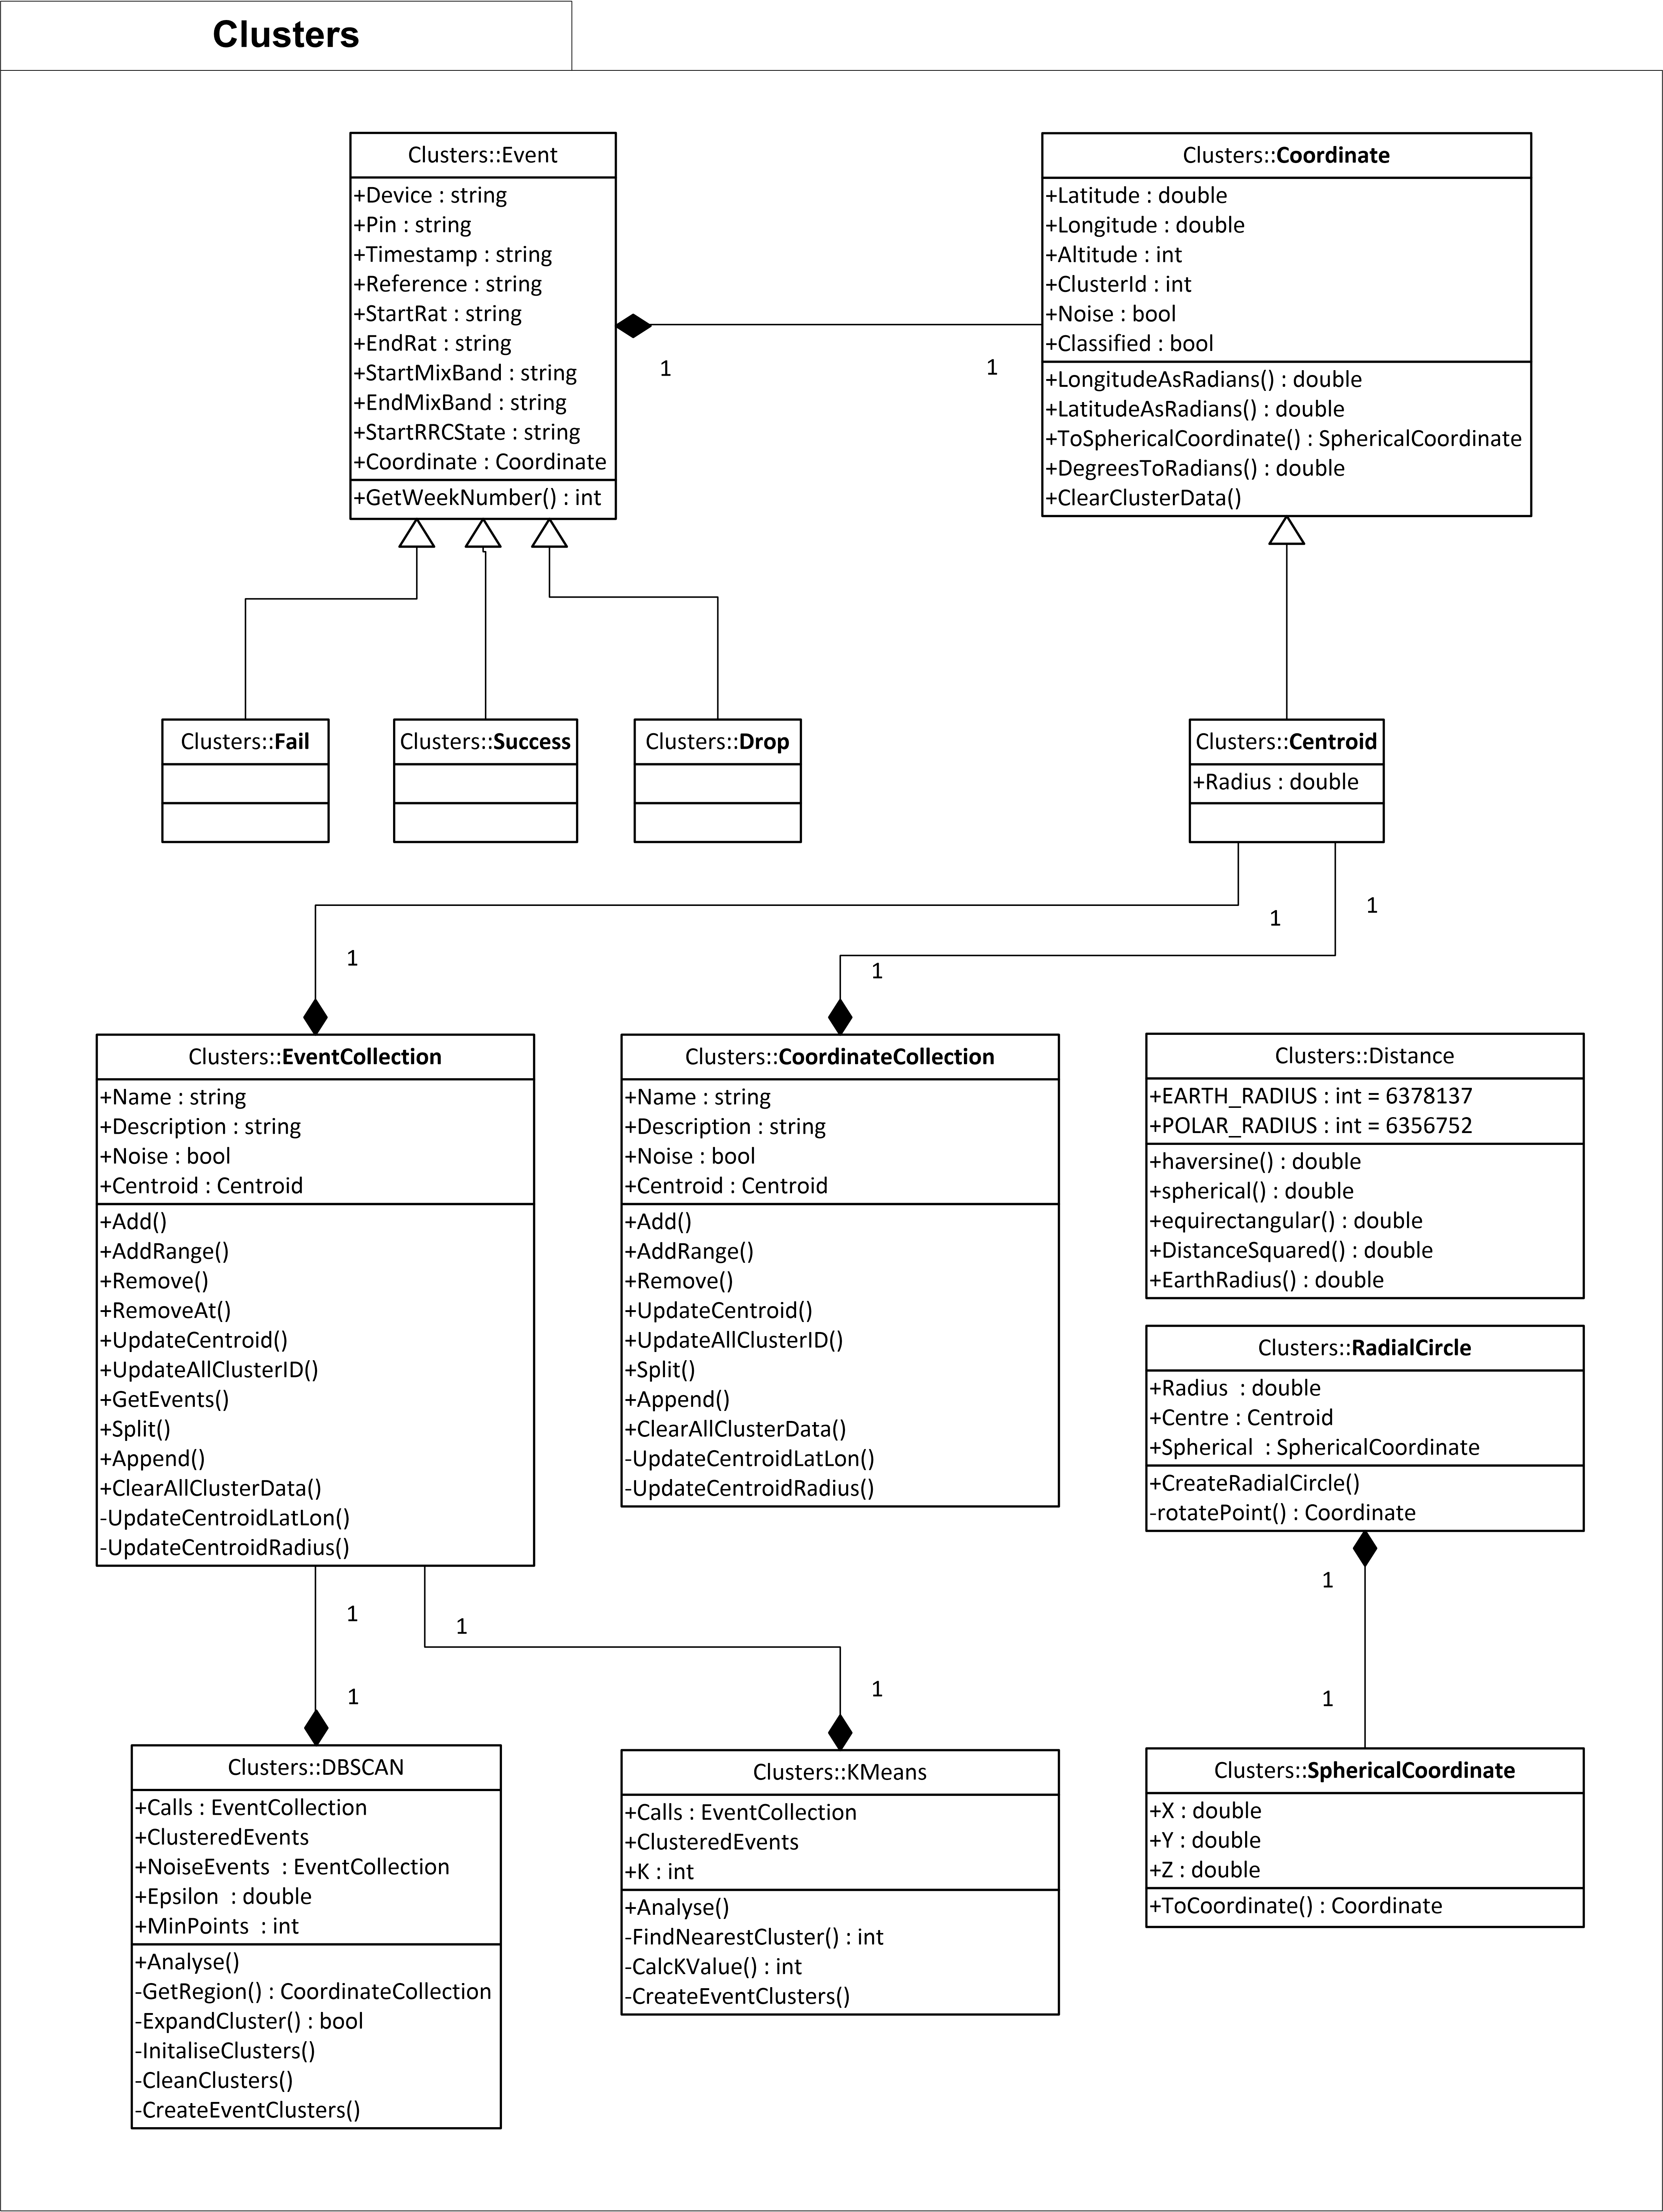
\includegraphics[scale=0.8]{chapter7/class_diagrams/clusters_namespace.png}
    \caption[Clusters namespace class diagram]
            {Clusters namespace class diagram.}
    \label{fig:NSClusters}
\end{figure}


\subsection{ClusterAnalysisTool}
Figure \ref{fig:NSClusterAnalysisTool} highlights the namespace that provides 
the main entry point to the tool. When complied this namespace will form an 
executable file (.exe) that allows the user to run the program via the command 
line. This is expressed in the Program file.

The Arguments class is a utility class for the Program file, which allows for 
easy parsing of (optionally) passed flags.

\begin{figure}[H]
  \centering
    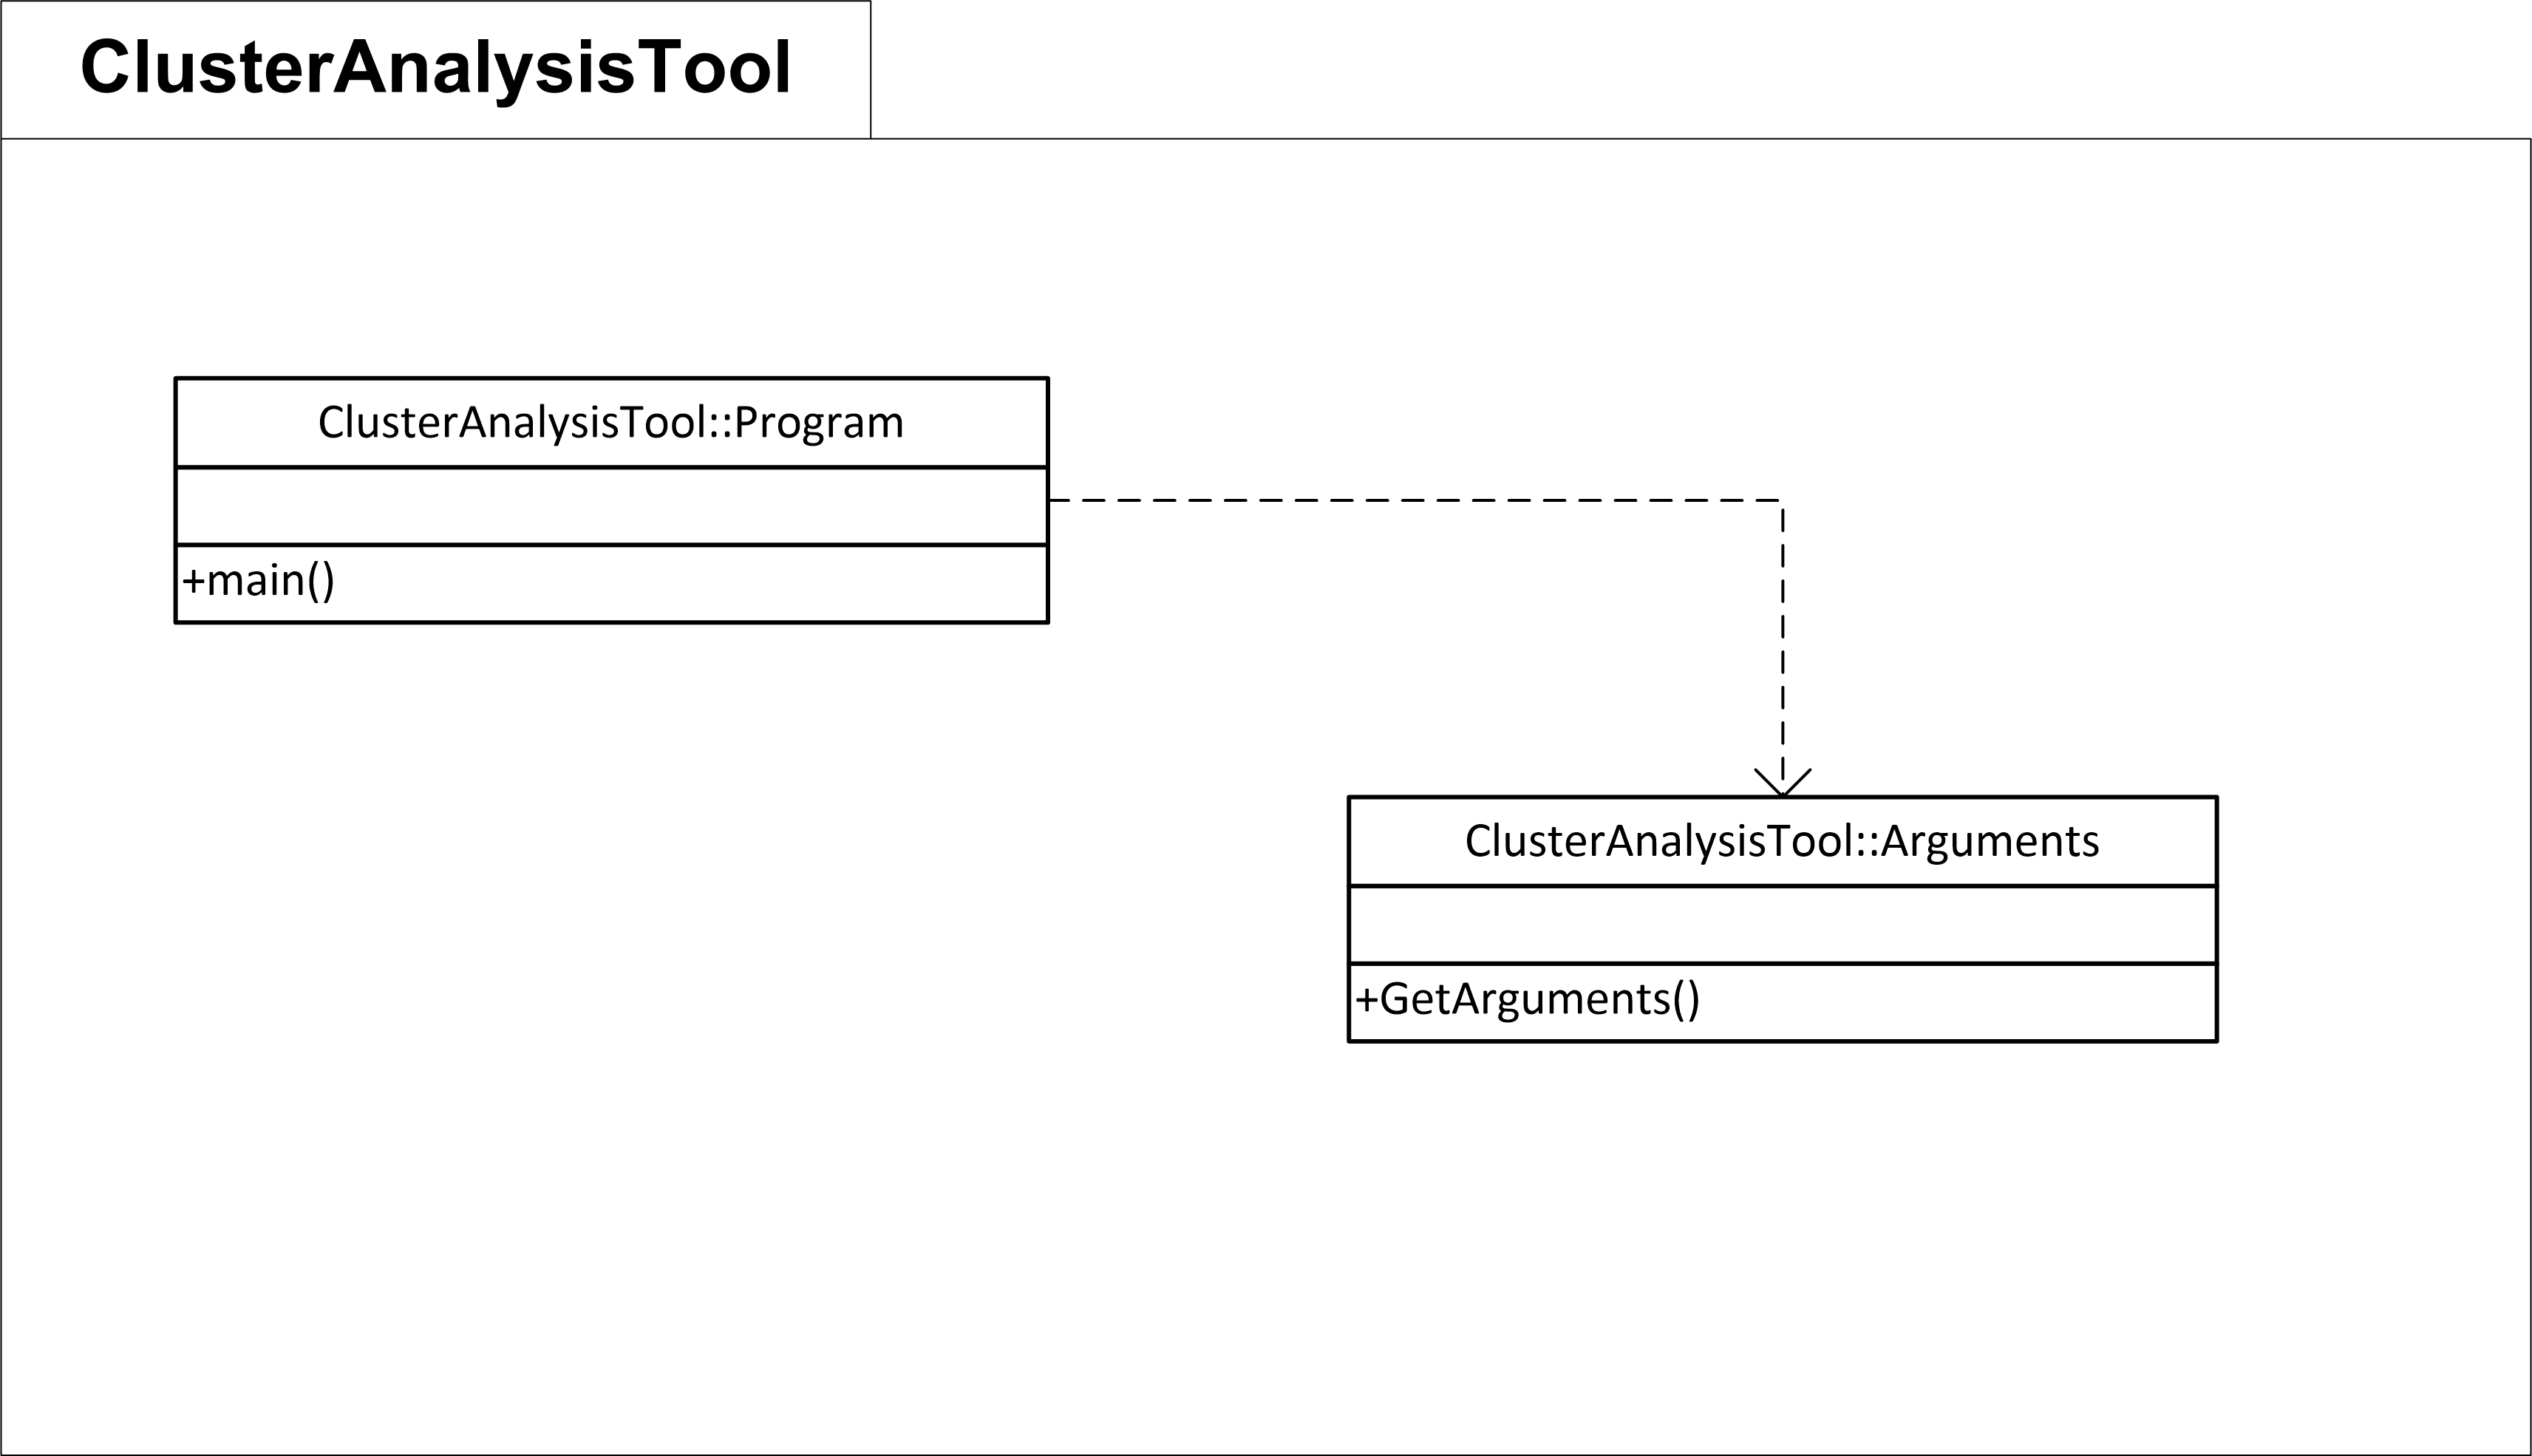
\includegraphics[scale=0.9]{chapter7/class_diagrams/clusteranalysistool_namespace.png}
    \caption[ClusterAnalysisTool namespace class diagram]
            {ClusterAnalysisTool namespace class diagram.}
    \label{fig:NSClusterAnalysisTool}
\end{figure}



\subsection{JSON}
Figure \ref{fig:NSJSON} highlights the namespace that handles creating well 
formed, sound JSON strings. This namespace, can be thought of a utility 
namespace.

This only class within this namespace, JSON, is a static class, and requires no 
instantiation. It creates a number of fundamental JSON strings, as well as 
being able to expand minified JSON code (referred to as prettify).

\begin{figure}[H]
  \centering
    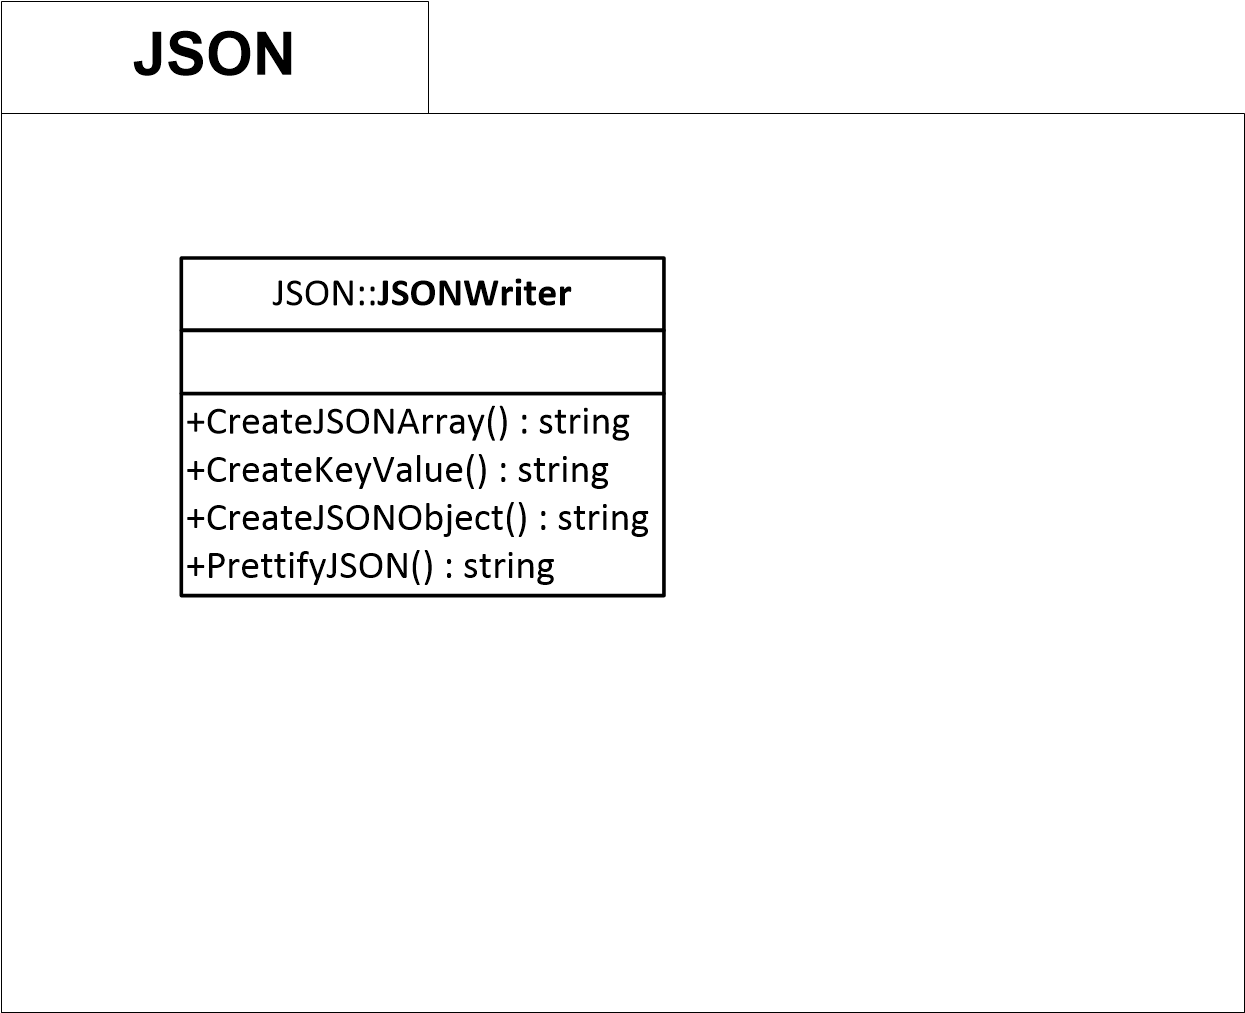
\includegraphics[scale=0.9]{chapter7/class_diagrams/json_namespace.png}
    \caption[JSON namespace class diagram]
            {JSON namespace class diagram.}
    \label{fig:NSJSON}
\end{figure}



\subsection{KML}
Figure \ref{fig:NSKML} highlights the namespace that handles the reading and 
writing of KML files. This namespace, like the JSON namespace, can be thought 
of a utility namespace.

The KML Writer class will create a well formed KML file, that can be opened 
from within Google Earth. 

The KML Reader class will read a KML file into an EventCollection object, which 
can be used in various other namespaces.

\begin{figure}[H]
  \centering
    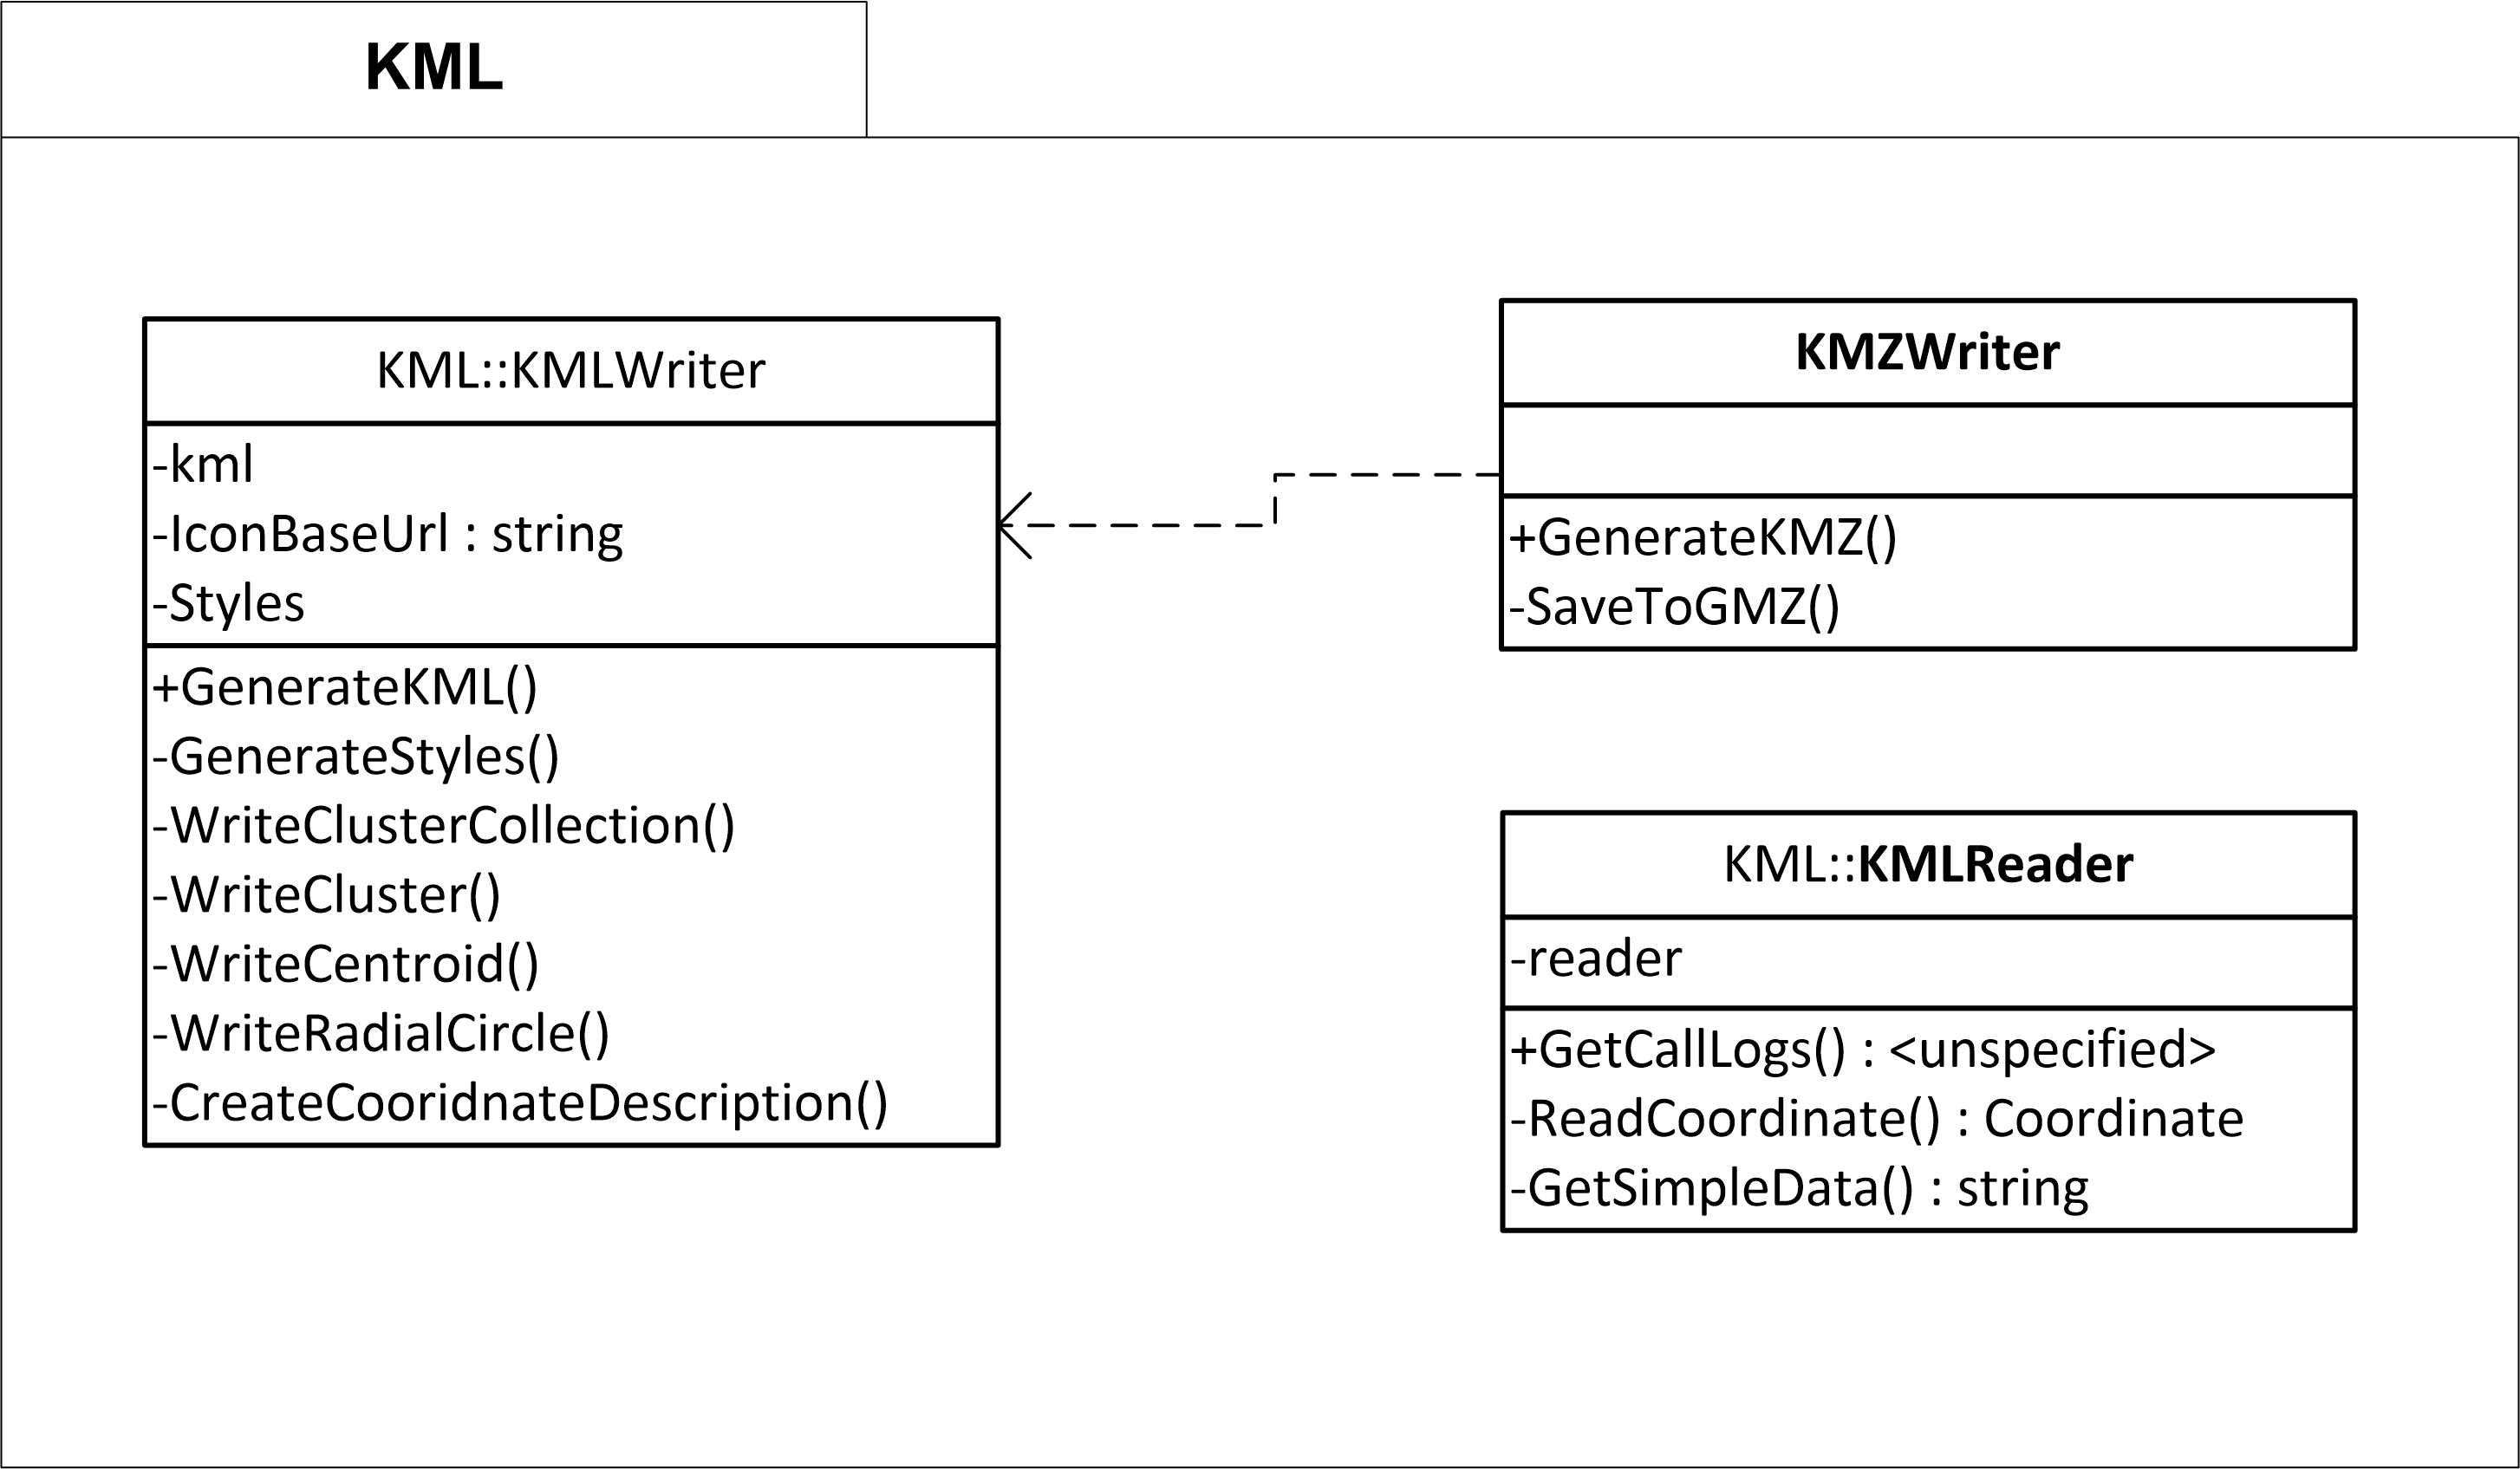
\includegraphics[scale=0.9]{chapter7/class_diagrams/kml_namespace.png}
    \caption[KML namespace class diagram]
            {KML namespace class diagram.}
    \label{fig:NSKML}
\end{figure}


